\tikzset{every picture/.style={line width=0.75pt}} %set default line width to 0.75pt        

\noindent
\begin{center}
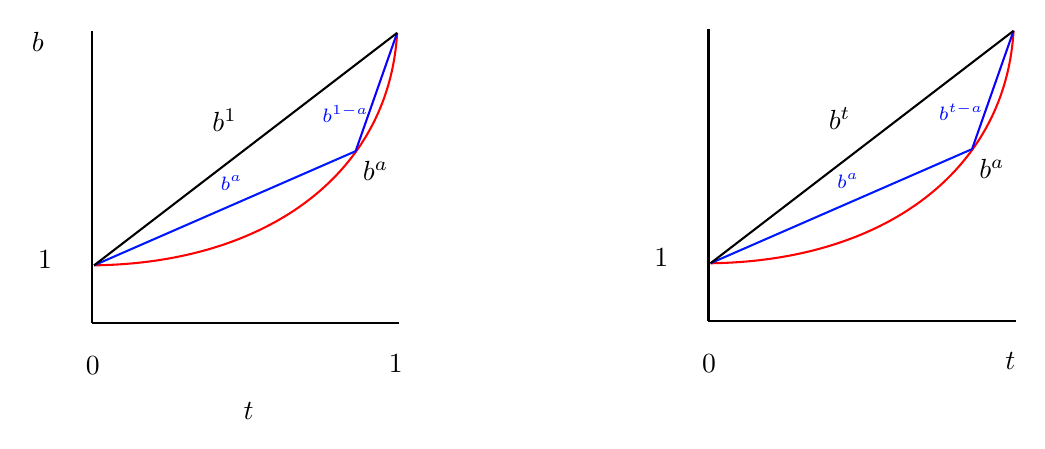
\begin{tikzpicture}[x=0.75pt,y=0.75pt,yscale=-1,xscale=1]
%uncomment if require: \path (0,300); %set diagram left start at 0, and has height of 300

%Curve Lines [id:da004250453094733597] 
\draw [color={rgb, 255:red, 255; green, 0; blue, 0 }  ,draw opacity=1 ]   (399.5,174) .. controls (482.5,173) and (541.5,130) .. (545.5,62) ;
%Straight Lines [id:da11185903183918833] 
\draw    (398.5,202) -- (546.5,202) ;
%Straight Lines [id:da2683371977344995] 
\draw    (398.5,61) -- (398.5,202) ;
%Straight Lines [id:da4582386497031067] 
\draw [color={rgb, 255:red, 0; green, 24; blue, 253 }  ,draw opacity=1 ]   (399.5,174) -- (525.5,119) ;
%Straight Lines [id:da2975129059808127] 
\draw [color={rgb, 255:red, 12; green, 0; blue, 255 }  ,draw opacity=1 ]   (545.5,62) -- (525.5,119) ;
%Straight Lines [id:da8666491434636445] 
\draw    (399.5,174) -- (545.5,62) ;
%Curve Lines [id:da8968805547814415] 
\draw [color={rgb, 255:red, 255; green, 0; blue, 0 }  ,draw opacity=1 ]   (102.5,175) .. controls (185.5,174) and (244.5,131) .. (248.5,63) ;
%Straight Lines [id:da4205745305765404] 
\draw    (101.5,203) -- (249.5,203) ;
%Straight Lines [id:da17942895279134785] 
\draw    (101.5,62) -- (101.5,203) ;
%Straight Lines [id:da8844445030454833] 
\draw [color={rgb, 255:red, 0; green, 24; blue, 253 }  ,draw opacity=1 ]   (102.5,175) -- (228.5,120) ;
%Straight Lines [id:da840463859307833] 
\draw [color={rgb, 255:red, 12; green, 0; blue, 255 }  ,draw opacity=1 ]   (248.5,63) -- (228.5,120) ;
%Straight Lines [id:da14755909330885852] 
\draw    (102.5,175) -- (248.5,63) ;

% Text Node
\draw (394,216.4) node [anchor=north west][inner sep=0.75pt]    {$0$};
% Text Node
\draw (540,215.4) node [anchor=north west][inner sep=0.75pt]    {$t$};
% Text Node
\draw (371,165.4) node [anchor=north west][inner sep=0.75pt]    {$1$};
% Text Node
\draw (527.5,122.4) node [anchor=north west][inner sep=0.75pt]    {$b^{a}$};
% Text Node
\draw (455,97.4) node [anchor=north west][inner sep=0.75pt]    {$b^{t}$};
% Text Node
\draw (459,129.4) node [anchor=north west][inner sep=0.75pt]  [font=\scriptsize,color={rgb, 255:red, 0; green, 15; blue, 255 }  ,opacity=1 ]  {$b^{a}$};
% Text Node
\draw (508,95.4) node [anchor=north west][inner sep=0.75pt]  [font=\scriptsize,color={rgb, 255:red, 0; green, 15; blue, 255 }  ,opacity=1 ]  {$b^{t-a}$};
% Text Node
\draw (97,217.4) node [anchor=north west][inner sep=0.75pt]    {$0$};
% Text Node
\draw (243,216.4) node [anchor=north west][inner sep=0.75pt]    {$1$};
% Text Node
\draw (74,166.4) node [anchor=north west][inner sep=0.75pt]    {$1$};
% Text Node
\draw (230.5,123.4) node [anchor=north west][inner sep=0.75pt]    {$b^{a}$};
% Text Node
\draw (158,98.4) node [anchor=north west][inner sep=0.75pt]    {$b^{1}$};
% Text Node
\draw (162,130.4) node [anchor=north west][inner sep=0.75pt]  [font=\scriptsize,color={rgb, 255:red, 0; green, 15; blue, 255 }  ,opacity=1 ]  {$b^{a}$};
% Text Node
\draw (211,96.4) node [anchor=north west][inner sep=0.75pt]  [font=\scriptsize,color={rgb, 255:red, 0; green, 15; blue, 255 }  ,opacity=1 ]  {$b^{1-a}$};
% Text Node
\draw (71,61.4) node [anchor=north west][inner sep=0.75pt]    {$b$};
% Text Node
\draw (173,239.4) node [anchor=north west][inner sep=0.75pt]    {$t$};


\end{tikzpicture}
\end{center}